%% The first command in your LaTeX source must be the \documentclass command.
%%
%% Options:
%% twocolumn : Two column layout.
%% hf: enable header and footer.
\documentclass[
    hf,
]{ceurart}
\usepackage[top=2.5cm, bottom=2.5cm, left=2.5cm, right=2.5cm]{geometry}

%%
%% One can fix some overfulls
\sloppy

%%
%% Minted listings support 
%% Need pygment <http://pygments.org/> <http://pypi.python.org/pypi/Pygments>
\usepackage{minted}
%% auto break lines
\setminted{breaklines=true}
\usepackage[utf8]{inputenc}	% allow utf-8 input
\usepackage{placeins} % for FloatBarrier
\usepackage{lipsum}
\usepackage{tabularx}
\usepackage{metrix}


%%
%% end of the preamble, start of the body of the document source.
\begin{document}

%%
%% Rights management information.
%% CC-BY is default license.
\copyrightyear{2024}
\copyrightclause{Copyright for this paper by its authors.
    Use permitted under Creative Commons License Attribution 4.0
    International (CC BY 4.0).}

%%
%% This command is for the conference information
% \conference{CHR 2022: Computational Humanities Research Conference, December 12 -- 14,
%     2022, Antwerp, Belgium}
\conference{}
%%
%% The "title" command
\title{Bootstrap Distance Imposters: A less accurate classifier for a more civilized age}

% \tnotemark[1]
% \tnotetext[1]{I would like to thank various members of the Computational
%     Stylistics Group \url{https://computationalstylistics.github.io/} for their
%     ideas and support}

%%
%% The "author" command and its associated commands are used to define
%% the authors and their affiliations.
\author[1]{Ben Nagy}[%
    orcid=0000-0002-5214-7595,
    url=https://github.com/bnagy/bdi-paper,
    email=benjamin.nagy@ijp.pan.pl,
]
\address[1]{Institute of Polish Language, Polish Academy of Sciences (IJP PAN)\\
    Adama Mickiewicz 31\\
    Kraków, Poland}
%%
%% The abstract is a short summary of the work to be presented in the
%% article.
\begin{abstract}
    I made a thing for authorship verification which has some nice properties.
\end{abstract}

%%
%% Keywords. The author(s) should pick words that accurately describe
%% the work being presented. Separate the keywords with commas.
\begin{keywords}
    authorship attribution \sep
    stylometry \sep
    bootstrapping \sep
\end{keywords}

%%
%% This command processes the author and affiliation and title
%% information and builds the first part of the formatted document.
\maketitle

\section{Introduction}

The General Imposters method (henceforth GI), originally formulated by M. Koppel
and Y. Winter in \cite{koppel_gi}, has become one of the standard
methods for authorship attribution. After strong performances in the PAN 2013 and
2014 competitions, it was implemented and used by M. Kestemont et al. in an
influential study \cite{kestemont_caesar}, improved by N. Potha and E.
Stamatatos in 2017 \cite{potha_improved_gi}, and is now available in the
well-known R package \emph{stylo} \cite{stylo}.

In this paper I describe an update to Kestemont's open-source Python
implementation called Bootstrap Distance Imposters (henceforth BDI) which
incorporates several of the improvements proposed since the last release, as
well as introducing a novel method of boostrapping that has several attractive
properties when compared to the reference algorithm. The two approaches are
benchmarked using the problems from the PAN 2014 author identification task
\cite{pan_2014}, and some additional properties are showcased via real-world
case studies.

\section{Motivation}
\begin{itemize}
    \item GI is more or less standard practice now
    \item the PAN 2014 competition is a convenient benchmark
    \item bootstrapped voting GI is not a measure of probability
    \item bootstrapped distance has several advantages
\end{itemize}
\section{Design}

The GI method is, in machine learning terms, an ensemble classifier. These
classifiers regularise well, but while they produce a real-valued output, it is
problematic to interpret this as a probability in any sense. The output of the
Kestemont GI classifier is a percentage of `votes' (the number of times a
candidate text was closer than an imposter). The score shifting method
implemented in Kestemont attempts to produce something more like a probability
by linearly scaling the output values. The scaling code (in Python) looks like this:
\begin{minted}{python}
    for score in list(scores):
        if score <= p1:
            new_scores.append(rescale(score, min(scores), max(scores), 0.0, p1))
        elif score >= p2:
            new_scores.append(rescale(score, min(scores), max(scores), p2, 1.0))
        else:
            new_scores.append(0.5)
\end{minted}

\cite{stover_kestemont_2016}
Scores below \mintinline{python}{p1} are scaled to the region up to
\mintinline{python}{p1}, scores above \mintinline{python}{p2} are scaled to the
region above \mintinline{python}{p2}, and the rest are coerced to 0.5. There is
an issue with this scaling algorithm, however. Since \mintinline{python}{p1} and
\mintinline{python}{p2} are arbitrarily chosen by grid search to maximise the
PAN score, the score shifter sometimes fits values for \mintinline{python}{p2}
that are well below 0.5. This can lead to decisions that should be positive
(since they are above \mintinline{python}{p2}) being scaled to below 0.5, where
they are evaluated by the scoring metrics as a negative result (and scored as
such). In the updated code I modified the shifting code to scale more simply to
$[0,0.5)$ 0.5 and $(0.5,1]$. This does not retain the global distributional
properties of the original results (as in Kestemont).

\begin{minted}{python}
    for score in scores:
            if score <= p1:
                new_scores.append(
                    rescale(score, orig_min=0, orig_max=p1, new_min=0.0, new_max=0.499)
                )
            elif score >= p2:
                new_scores.append(
                    rescale(score, orig_min=p2, orig_max=1, new_min=0.501, new_max=1.0)
                )
            else:
                new_scores.append(0.5)
\end{minted}

In contrast, the raw output from the BDI algorithm is a bootstrapped
distribution of differences. At each step, the distance (with this bootstrapped
feature set) between the candidates and the imposters is recorded. If the
candidates are further, the distance is negative, if closer it is positive. If
these individual distances follow a Gaussian distribution (which is a reasonable
prior expectation) then their difference is also Gaussian. Expressing the
results this way has some advantages. The first is that we can differentiate a
negative result (not the candidate) between `none of the above' and `more like
an imposter' (the true author is in the imposters set). A `none of the above'
result would have a statistically expected distance of zero (equally unlike the
candidate and the imposters), and so we would see a distribution centred around
0.%
%
\footnote{ Note carefully that this is a one-way implication---a true author
    that is neither the candidate nor one of the imposters should have a
    distance distribution centred around zero, but not all such distributions
    guarantee that the true author is not among the imposters.}
%
On the other hand, `more like an imposter' results show distributions centred
around a negative value. The other advantage is that for strong positives, we
have additional data about the match. Distributions centred around larger
positive numbers are better matches, but distributions with high variance show
more feature dependence (since the strength of the match varies greatly
depending on the bootstrap features). In summary, positive matches (with most or
all of the probability mass above zero) can be much more meaningfully compared.

Based on the BDI algorithm, which outputs a distribution, it is obviously useful
to have a summary statistic that can be interpreted as evidence for authorship
attribution tasks. For this paper I used a simple approach that considers the
amount of probability mass that lies above 0. If every test is closer to a
candidate that an imposter then the result will be 1, if every test is more like
an imposter, it will be 0, etc. This is implemented as
\mintinline{python}{(100-scipy.stats.percentileofscore(x, 0)) / 100.0}, the
inverse percentile of (a distance of) 0. Thus armed with a method that outputs a
`probability-like' result in $[0,1]$, I wrapped the code in a classifier that
follows \texttt{sklearn} conventions like \texttt{fit()} and
\texttt{predict\_proba()}  and evaluated the BDI classifier directly against the
updated Kestemont GI \texttt{Order2Verifier}, using the 2014 PAN authorship
attribution problems. This provided a convenient benchmark, and also the
opportunity to compare the results against a number of other (although older)
verification approaches.

\section{Classification Performance}

\subsection{Changes to Kestemont GI}

As is the nature of computing, the code in the repository documenting the GI
algorithm and for the related work on the Caesarian corpus no longer ran. I
reworked the code slightly, and made the following small changes, which are
available in my own repository.

\begin{itemize}
    \item Update the code to work with Python 3 (these minimal changes have been
          accepted into the original repository based on a PR)
    \item Implement the `nini' metric (fuzzy Jaccard similarity)
    \item Implement a partial version of the Potha \& Stamatatos `ranking'
          improvement for the consensus score%
          %
          \footnote{ Instead of a strict 1 (candidate closest) or 0 (candidate
              not closest), Potha \& Stamatatos proposed a score improvement
              based on the ordinal rank of the closest candidate, so if a
              candidate was the second-closest, the score for that iteration
              would be $\frac{1}{2}$. The same paper proposed a distance-based
              culling method to select more relevant imposters, but this was not
              implemented (with enough bootstrapping this should converge)}
          %
    \item Remove most non-core code
    \item Modify the score-shifting algorithm, as described above
\end{itemize}

\subsection{Testing}

\begin{table}
    \caption{Global micro-average results}
    \label{tab:micro}
    % \par\medskip
    \raggedright
    \begin{tabular}{lllcccc}
        \toprule
                                   &               &         & Accuracy       & AUC             & C@1            & Final Score    \\
        Classifier                 & Vectorizer    & Shifter &                &                 &                &                \\
        \midrule
        BDI, Cosine                & 2,3,4,5-grams & fitted  & 0.681          & 0.727           & 0.694          & 0.505          \\
                                   &               & manual  & 0.672          & 0.715           & 0.649          & 0.464          \\
                                   & 2,3,4-grams   & fitted  & 0.686          & 0.723           & 0.689          & 0.499          \\
                                   &               & manual  & 0.681          & 0.715           & 0.645          & 0.461          \\
        BDI, Minmax                & 2,3,4,5-grams & fitted  & \textbf{0.689} & 0.731           & 0.695          & 0.508          \\
                                   &               & manual  & 0.682          & 0.726           & 0.660          & 0.479          \\
                                   & 2,3,4-grams   & fitted  & 0.682          & 0.730           & 0.694          & 0.507          \\
                                   &               & manual  & 0.685          & 0.723           & 0.652          & 0.472          \\
        Kestemont GI, Cosine       & 2,3,4,5-grams & fitted  & 0.673          & 0.768           & 0.695          & 0.534          \\
                                   &               & manual  & 0.621          & 0.698           & 0.557          & 0.389          \\
                                   & 2,3,4-grams   & fitted  & 0.665          & 0.755           & 0.678          & 0.512          \\
                                   &               & manual  & 0.614          & 0.685           & 0.537          & 0.367          \\
        Kestemont GI, Minmax       & 2,3,4,5-grams & fitted  & 0.661          & \textbf{ 0.773} & \textbf{0.702} & \textbf{0.543} \\
                                   &               & manual  & 0.633          & 0.706           & 0.568          & 0.401          \\
                                   & 2,3,4-grams   & fitted  & 0.668          & 0.759           & 0.694          & 0.527          \\
                                   &               & manual  & 0.629          & 0.707           & 0.572          & 0.405          \\
        PAN 2014 Best (individual) &               &         & NA             & 0.718           & 0.684          & 0.490          \\
        \bottomrule
    \end{tabular}
\end{table}

\begin{table}
    \caption{BDI 2,3,4,5-grams, Minmax, Manual Shifter}
    \label{tab:bdi}
    % \par\medskip
    \raggedright
    \begin{tabular}{@{}lrrccccccc}
        \toprule
        Corpus       & Tests & ?? & High Conf. & FP & Acc  . & AUC   & C@1   & Final          & PAN Best       \\
        \midrule
        du\_essays   & 96    & 19 & 75         & 2  & 0.854  & 0.955 & 0.923 & \textbf{0.882} & 0.823          \\
        du\_reviews  & 50    & 10 & 35         & 0  & 0.580  & 0.693 & 0.576 & 0.399          & \textbf{0.525} \\
        en\_essays   & 200   & 27 & 162        & 0  & 0.605  & 0.624 & 0.568 & 0.354          & \textbf{0.513} \\
        en\_novels   & 200   & 34 & 161        & 0  & 0.595  & 0.622 & 0.556 & 0.346          & \textbf{0.508} \\
        gr\_articles & 100   & 34 & 61         & 2  & 0.800  & 0.848 & 0.697 & 0.591          & \textbf{0.720} \\
        sp\_articles & 100   & 35 & 53         & 1  & 0.780  & 0.882 & 0.810 & \textbf{0.715} & 0.698          \\
        \bottomrule
    \end{tabular}
\end{table}

\begin{table}
    \caption{Kestemont 2,3,4,5-grams, Minmax, Fitted Shifter}
    \label{tab:o2v}
    % \par\medskip
    \raggedright
    \begin{tabular}{lrrccccccc}
        \toprule
        Corpus       & Tests & ?? & High Conf. & FP & Acc  . & AUC   & C@1   & Final          & PAN Best       \\
        \midrule
        du\_essays   & 96    & 16 & 54         & 2  & 0.854  & 0.964 & 0.948 & \textbf{0.914} & 0.823          \\
        du\_reviews  & 50    & 12 & 14         & 7  & 0.640  & 0.696 & 0.645 & 0.449          & \textbf{0.525} \\
        en\_essays   & 200   & 14 & 22         & 73 & 0.565  & 0.569 & 0.578 & 0.329          & \textbf{0.513} \\
        en\_novels   & 200   & 42 & 79         & 12 & 0.610  & 0.670 & 0.629 & 0.421          & \textbf{0.508} \\
        gr\_articles & 100   & 28 & 18         & 3  & 0.790  & 0.840 & 0.755 & 0.634          & \textbf{0.720} \\
        sp\_articles & 100   & 15 & 27         & 6  & 0.750  & 0.935 & 0.863 & \textbf{0.807} & 0.698          \\
        \bottomrule
    \end{tabular}
\end{table}

\begin{figure*}
    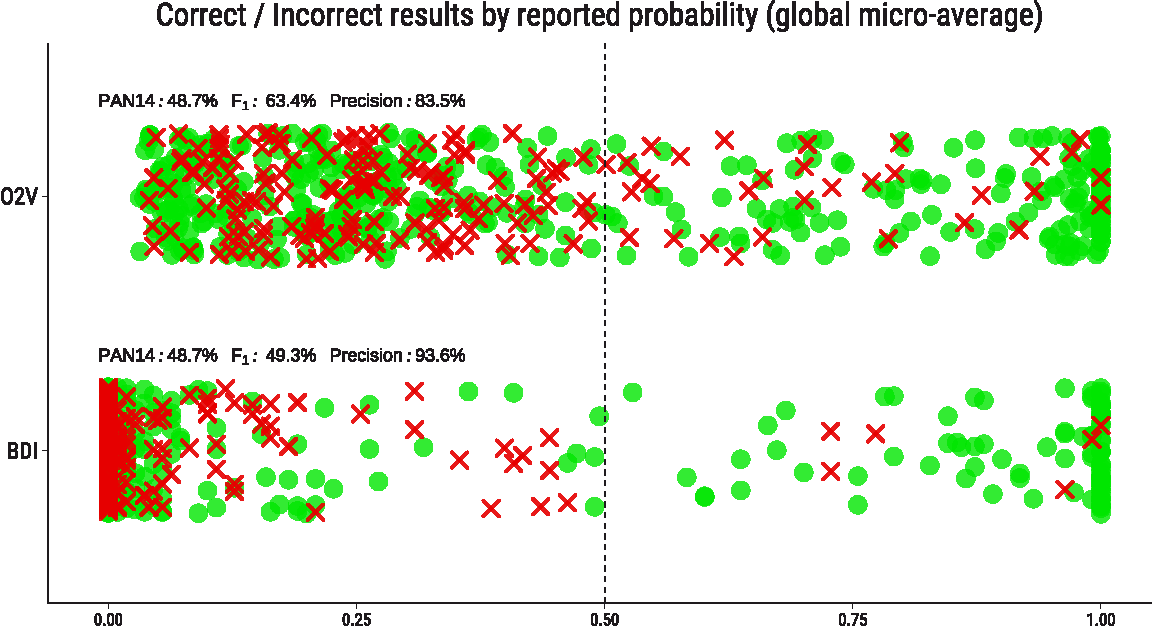
\includegraphics[width=\linewidth]{figures/bdi_o2v-crop.pdf}
    \caption{A comparison of the correct and incorrect results by reported
        probability for BDI (manual shifter, 2,3,4,5-grams, minmax) vs
        Order2Verifer (fitted shifter, 2,3,4,5-grams, minmax)}
    \label{fig:bdi_o2v}
\end{figure*}


The BDI classifier was compared head-to-head with the updated Kestemont
\texttt{Order2Verifier} on the full PAN 2014 evaluation corpus, as archived in
the github repository.%
%
\footnote{ There is a small inconsistency that I was unable to resolve---the
    verification problems stored at the Kestemont repository are apparently
    missing 50 of the `Dutch Reviews' evaluation problems, so there are a total
    of 746, versus 796 reported in the PAN 2014 wrapup report.
}
%
For this test I used two different sets of character $n$-grams, since that
feature universe is a generally reliable and uncontroversial choice for modern
authorship-attribution work. There may be feature universes that perform better,
or features that work better for a specific task, but character $n$-grams are
`solid if boring'. Likewise, the $n$-gram frequencies are $z$-scaled (based on
the training variances) since this is the `standard' approach. I tested two
$n$-gram configurations, 2,3,4-grams and 2,3,4,5-grams, with fitted and manual
score shifting. Finally, for the distance metric used to determine `closeness'
at each step I tested the cosine distance (the most traditional choice) and the
minmax (Ružička) metric promoted by Kestemont in his original paper. Consistent
with those results, the minmax metric appears generally superior (see Table
\ref{tab:micro}). The fully reproducible testing code is available in the
supplementary repository.

\subsection{Interpretation}

As can be seen from Table \ref{tab:micro}, the performance of the BDI classifier
is consistently strong, with only a small boost in PAN score resulting from
fitting the score shifter. The GI \texttt{Order2Verifier} with a fitted shifter
performs better according to the PAN metrics (deriving a large c@1 benefit from
fitting the score shifter). The GI classifier also appears to outperform the
best overall PAN 2014 entrant by a significant margin. The strength of the BDI
classifiers, however, is twofold: first, they do not really require any training
corpus, and second, the BDI approach is high precision (it yields very few false
positives), making it a conservative classifier whose positive results are
reliable (at the cost of more false negatives). This can be seen clearly in
Figure \ref{fig:bdi_o2v} in which the best performing GI classifier is compared
to the unfitted BDI classifier, using the same features and metrics. The results
for each subcorpus are broken down in more detail in Tables \ref{tab:bdi} \&
\ref{tab:o2v}.

\section{Results}
\begin{itemize}
    \item BDI is more understandable (<0\% or >100\%)
    \item Doesn't need score shifting
    \item Fewer false positives
    \item Summary stat still works as a classifier
\end{itemize}
\section{Future Work}
\section{Conclusions}

\section{Availability of Data and Code}\label{sec:data}

The preprint may be found at \url{https://github.com/bnagy/bdi-paper}. All code
and data is available under CC-BY, except where restricted by upstream licenses.
The code repository includes all of the source data, the saved models, and
Python notebooks to replicate all figures contained in this paper, as well as
various supplemental figures and explanations.

%%
%% The acknowledgments section is defined using the "acknowledgments" environment
%% (and NOT an unnumbered section). This ensures the proper
%% identification of the section in the article metadata, and the
%% consistent spelling of the heading.
\begin{acknowledgments}
    This work was supported by Polish Academy of Sciences Grant
    2020/39 / O / HS2 / 02931.
\end{acknowledgments}

%%
%% Define the bibliography file to be used
\bibliography{digilat}

%%
%% If your work has an appendix, this is the place to put it.
\appendix
\onecolumn

\end{document}

%%
%% End of file